\chapter{Classical Background}

\section{Euler-Bernoulli Beam Theory}
%
The simplest representation of bending behavior is found in the Euler-Bernoulli beam equation (\cref{eq:EulerBeam}), which describes the transverse deflection of long-slender beams.
\begin{equation}
\label{eq:EulerBeam}
\frac{\text{d}^2}{\text{d}x^2}\left(EI\frac{\text{d}^2 v}{\text{d} x^2}\right) = q
\end{equation}
The equation is for a beam in the $\hat{x}$ direction, whose displacement $v$ is perpendicular to $\hat{x}$ and parallel to the distributed load $q$ acting on the beam.
While it is only applicable to small deformations and rotations, there are many problems that can be easily and usefully simplified by the application of Euler beams.

It is important to note that \cref{eq:EulerBeam} is not a constitutive equation; it does not relate stress and strain for a material. 
Instead, it is derived from the constitutive equation for a linearly-elastic material and some assumptions about the deformation.
Euler-Bernoulli beam theory is much simpler than a 3D analysis of a beam as a solid material, but it requires the following assumptions to be met:
\begin{itemize}
 \item Slenderness: the length of the beam should be 20 times its other dimensions
 \item Loaded transversely, no axial loads or torques
 \item Small deformations and rotations
 \item Plane cross-sections of the beam remain plane under deformation
 \item Initially straight, and symmetric about the plane of bending
\end{itemize}
First, we take a infinitesimal slice of a beam as depicted in \cref{fig:Infinitesimal}.
Because we will want to compare to this model later, we use a different $y$-coordinate direction than many presentations.
We use this infinitesimal slice to derive the relationship between load, shear, and moment.

%
\begin{figure}[htbp]
  \centering
  


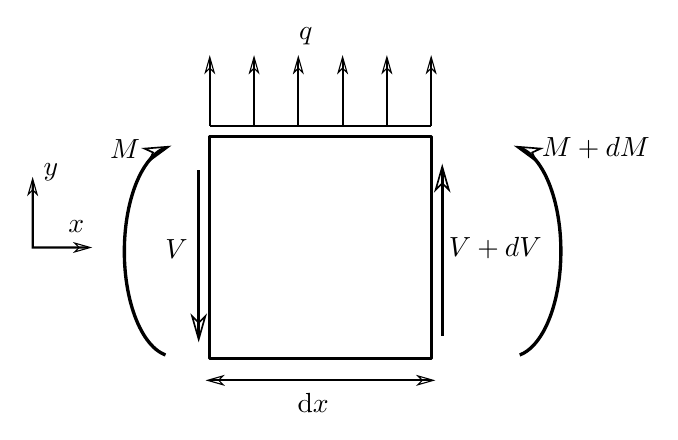
\begin{tikzpicture}[y=0.80pt, x=0.8pt,yscale=-1, inner sep=0pt, outer sep=0pt]
\begin{scope}[shift={(0,-752.36218)}]
  \path[draw=black,fill=black,line join=round,miter limit=4.00,fill
    opacity=0.000,nonzero rule,line width=1.200pt,rounded corners=0.0000cm]
    (95.0000,852.3622) rectangle (195.0000,952.3622);
    \path[color=black,fill=black,line width=0.800pt] (95.0000,961.8750) --
      (95.0000,962.8750) -- (195.0000,962.8750) -- (195.0000,961.8750) --
      (95.0000,961.8750) -- cycle;
    \path[draw=black,even odd rule,line width=0.400pt] (99.0000,962.3622) --
      (101.0000,960.3622) -- (94.0000,962.3622) -- (101.0000,964.3622) --
      (99.0000,962.3622) -- cycle;
    \path[draw=black,even odd rule,line width=0.400pt] (191.0000,962.3622) --
      (189.0000,964.3622) -- (196.0000,962.3622) -- (189.0000,960.3622) --
      (191.0000,962.3622) -- cycle;
    \path[color=black,fill=black,line width=1.200pt] (199.2500,867.3750) --
      (199.2500,942.3750) -- (200.7500,942.3750) -- (200.7500,867.3750) --
      (199.2500,867.3750) -- cycle;
    \path[draw=black,even odd rule,line width=0.600pt] (200.0000,873.3622) --
      (203.0000,876.3622) -- (200.0000,865.8622) -- (197.0000,876.3622) --
      (200.0000,873.3622) -- cycle;
    \path[color=black,fill=black,line width=1.200pt] (89.2500,867.3750) --
      (89.2500,942.3750) -- (90.7500,942.3750) -- (90.7500,867.3750) --
      (89.2500,867.3750) -- cycle;
    \path[draw=black,even odd rule,line width=0.600pt] (90.0000,936.3622) --
      (87.0000,933.3622) -- (90.0000,943.8622) -- (93.0000,933.3622) --
      (90.0000,936.3622) -- cycle;
    \path[color=black,fill=black,nonzero rule,line width=1.200pt] (74.7508,856.6718)
      .. controls (69.8130,858.5099) and (65.5561,863.3884) .. (62.3133,870.2343) ..
      controls (59.0705,877.0802) and (56.8284,885.9197) .. (56.0008,895.8280) ..
      controls (54.9137,908.8435) and (56.4098,921.5363) .. (59.7508,931.6093) ..
      controls (63.0918,941.6823) and (68.2689,949.1964) .. (74.7508,951.6093) --
      (75.2508,950.2030) .. controls (69.4951,948.0605) and (64.4529,940.9833) ..
      (61.1883,931.1405) .. controls (57.9237,921.2978) and (56.4301,908.7726) ..
      (57.5008,895.9530) .. controls (58.3158,886.1958) and (60.5450,877.4952) ..
      (63.6883,870.8593) .. controls (66.8316,864.2234) and (70.8734,859.7075) ..
      (75.2508,858.0780) -- (74.7508,856.6718) -- cycle;
    \path[draw=black,even odd rule,line width=0.600pt] (69.3769,859.4553) --
      (67.6120,863.3134) -- (76.4058,856.8389) -- (65.5188,857.6904) --
      (69.3769,859.4553) -- cycle;
    \path[color=black,fill=black,nonzero rule,line width=1.200pt]
      (235.2492,856.6718) -- (234.7492,858.0780) .. controls (240.5049,860.2206) and
      (245.5471,867.2978) .. (248.8117,877.1405) .. controls (252.0763,886.9833) and
      (253.5699,899.5085) .. (252.4992,912.3280) .. controls (251.6842,922.0852) and
      (249.4550,930.7859) .. (246.3117,937.4218) .. controls (243.1684,944.0577) and
      (239.1266,948.5735) .. (234.7492,950.2030) -- (235.2492,951.6093) .. controls
      (240.1869,949.7712) and (244.4439,944.8927) .. (247.6867,938.0468) .. controls
      (250.9295,931.2009) and (253.1716,922.3614) .. (253.9992,912.4530) .. controls
      (255.0863,899.4376) and (253.5902,886.7448) .. (250.2492,876.6718) .. controls
      (246.9082,866.5988) and (241.7311,859.0847) .. (235.2492,856.6718) -- cycle;
    \path[draw=black,even odd rule,line width=0.600pt] (240.6231,859.4553) --
      (244.4812,857.6904) -- (233.5942,856.8389) -- (242.3880,863.3134) --
      (240.6231,859.4553) -- cycle;
  \path[fill=black] (134.65359,976.70172) node[above right] (text7264) {d$x$};
  \path[fill=black] (75,907.36218) node[above right] (text7268) {$V$};
  \path[fill=black] (50,862.36218) node[above right] (text7272) {$M$};
  \path[fill=black] (203,907.36218) node[above right] (text7276) {$V+\text{d}V$};
  \path[fill=black] (245,862.36218) node[above right] (text7280) {$M+\text{d}M$};
  \path[draw=black,line join=miter,line cap=butt,line width=0.800pt]
    (95.0000,847.3622) -- (195.0000,847.3622);
    \path[color=black,fill=black,line width=0.800pt] (94.5000,817.3750) --
      (94.5000,847.3750) -- (95.5000,847.3750) -- (95.5000,817.3750) --
      (94.5000,817.3750) -- cycle;
    \path[draw=black,even odd rule,line width=0.400pt] (95.0000,821.3622) --
      (97.0000,823.3622) -- (95.0000,816.3622) -- (93.0000,823.3622) --
      (95.0000,821.3622) -- cycle;
    \path[color=black,fill=black,line width=0.800pt] (174.5000,817.3750) --
      (174.5000,847.3750) -- (175.5000,847.3750) -- (175.5000,817.3750) --
      (174.5000,817.3750) -- cycle;
    \path[draw=black,even odd rule,line width=0.400pt] (175.0000,821.3622) --
      (177.0000,823.3622) -- (175.0000,816.3622) -- (173.0000,823.3622) --
      (175.0000,821.3622) -- cycle;
    \path[color=black,fill=black,line width=0.800pt] (114.5000,817.3750) --
      (114.5000,847.3750) -- (115.5000,847.3750) -- (115.5000,817.3750) --
      (114.5000,817.3750) -- cycle;
    \path[draw=black,even odd rule,line width=0.400pt] (115.0000,821.3622) --
      (117.0000,823.3622) -- (115.0000,816.3622) -- (113.0000,823.3622) --
      (115.0000,821.3622) -- cycle;
    \path[color=black,fill=black,line width=0.800pt] (134.5000,817.3750) --
      (134.5000,847.3750) -- (135.5000,847.3750) -- (135.5000,817.3750) --
      (134.5000,817.3750) -- cycle;
    \path[draw=black,even odd rule,line width=0.400pt] (135.0000,821.3622) --
      (137.0000,823.3622) -- (135.0000,816.3622) -- (133.0000,823.3622) --
      (135.0000,821.3622) -- cycle;
    \path[color=black,fill=black,line width=0.800pt] (194.5000,817.3750) --
      (194.5000,847.3750) -- (195.5000,847.3750) -- (195.5000,817.3750) --
      (194.5000,817.3750) -- cycle;
    \path[draw=black,even odd rule,line width=0.400pt] (195.0000,821.3622) --
      (197.0000,823.3622) -- (195.0000,816.3622) -- (193.0000,823.3622) --
      (195.0000,821.3622) -- cycle;
    \path[color=black,fill=black,line width=0.800pt] (154.5000,817.3750) --
      (154.5000,847.3750) -- (155.5000,847.3750) -- (155.5000,817.3750) --
      (154.5000,817.3750) -- cycle;
    \path[draw=black,even odd rule,line width=0.400pt] (155.0000,821.3622) --
      (157.0000,823.3622) -- (155.0000,816.3622) -- (153.0000,823.3622) --
      (155.0000,821.3622) -- cycle;
  \path[fill=black] (135.3607,810.88519) node[above right] (text7684) {$q$};
    \path[color=black,fill=black,line width=0.800pt] (14.5000,872.3622) --
      (14.5000,902.3622) -- (14.5000,902.8622) -- (15.0000,902.8622) --
      (40.0000,902.8622) -- (40.0000,901.8622) -- (15.5000,901.8622) --
      (15.5000,872.3622) -- (14.5000,872.3622) -- cycle;
    \path[draw=black,even odd rule,line width=0.400pt] (36.0000,902.3622) --
      (34.0000,904.3622) -- (41.0000,902.3622) -- (34.0000,900.3622) --
      (36.0000,902.3622) -- cycle;
    \path[draw=black,even odd rule,line width=0.400pt] (15.0000,876.3622) --
      (17.0000,878.3622) -- (15.0000,871.3622) -- (13.0000,878.3622) --
      (15.0000,876.3622) -- cycle;
  \path[shift={(0,752.36218)},fill=black] (31.112698,143.02229) node[above right]
    (text9186) {$x$};
  \path[fill=black] (20,872.36218) node[above right] (text9190) {$y$};
\end{scope}

\end{tikzpicture}


  \caption{Infinitesimal Beam Slice}
  \label{fig:Infinitesimal}
\end{figure}
%
\todo{Where are your arrows on the figure}. A force balance demonstrates that the x-derivative of internal shear force is the applied load:
\begin{equation}
\label{eq:EulerShear}
V = V + q\;\text{d}x + \text{d}V \implies \frac{\text{d}V}{\text{d}x} = -q
\end{equation}
The moment balance can be performed about any point, but it is simplest to use the right side:
\begin{equation}
\label{eq:EulerMoment}
M - V\text{d}x +q\;\text{d}x\frac{\text{d}x}{2} = M + \text{d}M \implies \frac{\text{d} M}{\text{d}x} = -V + \mathcal{O}(\text{d}x)
\end{equation}


Next, we will use the deformation assumptions to frame the bending as a simple arc
%
\begin{figure}[htbp]
  \centering
  


\begin{tikzpicture}[y=0.80pt, x=0.8pt,yscale=-1, inner sep=0pt, outer sep=0pt]
  \path[draw=black,miter limit=4.00,line width=1.200pt]
    (15.2615,55.3504)arc(260.000:289.500:200.051);
  \path[draw=black,line join=round,miter limit=4.00,line width=1.200pt]
    (6.4976,5.6478)arc(260.000:290.000:250.520);
  \path[draw=black,dash pattern=on 2.40pt off 0.80pt,line join=round,miter
    limit=4.00,line width=0.800pt] (11.7974,30.7804)arc(260.000:290.000:220.000000
    and 225.000);
  \path[draw=black,line join=miter,line cap=butt,line width=0.800pt]
    (50.0000,232.3622) -- (10.0000,32.3622);
  \path[draw=black,line join=miter,line cap=butt,line width=0.800pt]
    (50.0000,27.3622) -- (35.0000,52.3622) -- (50.0000,52.3622) --
    (50.0000,2.3622) -- (65.0000,2.3622) -- cycle;
  \path[fill=black] (29.7995,97.515488) node[above right] (text8240) {\(\rho =
    \sfrac{1}{\kappa}\)};
  \path[fill=black] (65,22.362183) node[above right] (text8248) {\(\epsilon = -y
    \kappa\)};
  \path[draw=black,line join=miter,line cap=butt,line width=0.800pt]
    (50.0000,232.3622) -- (125.0000,42.3622);
  \path[cm={{0.4407,0.0,0.0,0.4407,(27.965,129.30866)}},draw=black,miter
    limit=4.00,line width=1.200pt] (15.2615,55.3504)arc(260.000:289.500:200.051);
  \path[fill=black] (45,147.36218) node[above right] (text3984) {d$\theta$};
  \path[fill=black] (115,32.362183) node[above right] (text3988) {d$s$};

\end{tikzpicture}


  \caption{Small deformation in an Euler beam}
  \label{fig:EulerBeam1}
\end{figure}
%
from which we can deduce a relationship between the transverse displacement of a beam section and its angle and radius of curvature. \todo{I just noticed this, but your equations need to be punctuated like they are part of a sentence}
\begin{equation}
 \label{eq:EulerCurve}
 \frac{1}{\rho} \approx \frac{\text{d} \theta}{\text{d} x} \approx \frac{\text{d}^2v}{\text{d}x^2} = \kappa
\end{equation}
The radius of curvature, $\rho$ is the radius of the arc formed by the beam's neutral axis, which does not change in length as the beam bends.
We use this same arc to find the strain in material that is at a distance $y$ from the neutral axis.
In a linearly elastic material, the resulting stress is proportional to Young's modulus $E$.
To find the bending moment that results from that stress profile, we integrate the moment contribution through the beam.
\begin{equation}
M_\text{resisted} = \int_\text{bottom}^\text{top}y\sigma dA = \int_\text{bottom}^\text{top}y^2 E \kappa dA
\end{equation}
In equilibrium, the moment resisted will be equal and opposite to the moment applied.
\begin{equation}
\label{eq:MomentCurve}
\kappa = \frac{M_\text{applied}}{E \int_\text{bottom}^\text{top}y^2dA}
\end{equation}
The integral in the denominator is the bending resistance of the beam's shape, called its second moment of area, about the neutral axis.
The second moment of area is generally represented by $I$.
By combining \cref{eq:EulerShear,eq:EulerMoment,eq:EulerCurve,eq:MomentCurve}, we reproduce  \cref{eq:EulerBeam}, the Euler-Bernoulli beam equation.
If the Young's modulus and beam cross section are constant throughout the beam, the equation can be further simplified to
\begin{equation}
EI\frac{\text{d}^4 v}{\text{d}x^4}=q\notag
\end{equation}

Obviously, to solve for the deformed position we will require 4 constraints from boundary conditions.
The nature of the constraints is determined by the support configuration.
The most common end conditions are listed \cref{table:BeamBCs}.
Other end constraints, such 

\begin{table}
\centering
\begin{tabular}{l >{$\displaystyle}l<{$} >{$\displaystyle}l<{$}}
End Condition & \textrm{Contraint 1} & \textrm{Constraint 2}\\ \hline\hline
End Load & v'''=\pm F  &  v''=0  \\ \hline
End Torque & v'''=0  &  v''= \pm \tau  \\ \hline
Simply Supported & v''=0 & v=v_\text{support}  \\ \hline
Clamped & v'=v'_\text{clamp} & v=v_\text{clamp}  \\ \hline\hline
\end{tabular}
\caption{Common Beam End Conditions}
\label{table:BeamBCs}
\end{table}

\section{Kirchhoff-Love Plate Theory}
Like Euler-Bernoulli beam theory, Kirchhoff-Love Plate theory begins by making simplifying assumptions about the plate and its deformation.
\begin{itemize}
 \item Slenderness: the length and width of the plate should be 20 times its thickness
 \item Loaded transversely, no in-plane loads or torques
 \item Small deformations and rotations
 \item Straight lines normal to the plate remain normal to the center plane of the plate under deformation
 \item Initially flat
\end{itemize}
These assumptions allow us to simplify our strain-displacement relationships and formulate our curvatures and strains in terms of the transverse displacement $w$.
\begin{equation}
    \kappa_x=\frac{\partial^2 w}{\partial x^2}, \quad \kappa_y= \frac{\partial^2 w}{\partial y^2}, \quad \kappa_{xy}=\frac{\partial^2 w}{\partial x\partial y}\notag
\end{equation}
\begin{equation}
\varepsilon_x = -z \kappa_x, \quad \varepsilon_y = -z \kappa_y, \quad \gamma_{xy} = -2 z \kappa_{xy} \notag
\end{equation}
To find the stresses at any point, we apply Hooke's law and find
\begin{align*}
\sigma_x &= -\frac{E z}{1-\nu^2}\left(\kappa_x+\nu\kappa_y\right)\\
\sigma_y &= -\frac{E z}{1-\nu^2}\left(\kappa_y+\nu\kappa_x\right)\\
\tau_{xy} &= -\frac{Ez}{1+\nu}\kappa_{xy}
\end{align*}
As with the beam, these stresses can be integrated over the thickness of the plate to determine the resulting moments.
\begin{align*}
M_x = \int_{\sfrac{-t}{2}}^{\sfrac{t}{2}}z\sigma_x dz &=-D\left(\kappa_x+\nu\kappa_y\right)\\
M_y = \int_{\sfrac{-t}{2}}^{\sfrac{t}{2}}z\sigma_y dz &=-D\left(\kappa_y+\nu\kappa_x\right)\\
M_{xy} = \int_{\sfrac{-t}{2}}^{\sfrac{t}{2}}z\tau_{xy}dz &= -D\left(1-\nu\right)\kappa_{xy}
\end{align*}
with
\begin{equation*}
D=\frac{Et^3}{12\left(1-\nu^2\right)}
\end{equation*}
as the flexural rigidity.

Constructing the governing equation is more complicated than for beams because, instead of shear $V$ and moment $M$ on an infinitesimal section, we have shears $V_x$ and $V_y$ and moments $M_x$, $M_y$, and $M_{xy}$.
Balancing forces gives us
\begin{equation}
\frac{\partial V_x}{\partial x}+\frac{\partial V_y}{\partial y} = p
\end{equation}
for transverse pressure $p$.
Balancing moments gives
\begin{align}
\text{about} \;x:\qquad& \frac{\partial M_{xy}}{\partial x}+\frac{\partial M_{y}}{\partial y} - V_y = 0\\
\text{about} \;y:\qquad& \frac{\partial M_{xy}}{\partial y}+\frac{\partial M_{x}}{\partial x} - V_x = 0
\end{align}

Combining the force and moment balance equations generates the governing equation
\begin{equation}
\frac{\partial^4w}{\partial x^4}+2\frac{\partial^4w}{\partial x^2 \partial y^2}+\frac{\partial^4w}{\partial y^4}=\frac{p}{D}
\end{equation}
As with the beam case, we will need to apply boundary conditions in order to find the deformed configuration.
